% !TEX encoding = UTF-8 Unicode
% !TEX TS-program = pdflatex
% !TEX spellcheck = it-IT
\documentclass[a4paper,titlepage]{article}

\usepackage[utf8x]{inputenc}
\usepackage{eurosym}
\usepackage{hyperref}

\makeatletter
\def\input@path{{../../../template/}}
\makeatother

\usepackage{Comandi}
\usepackage{Riferimenti}
\usepackage{Stile}


%Nome del documento
\def\NOME{Piano di Qualifica}
%Versione del documento
\def\VERSIONE{3.0.0}
%Data del documento
\def\DATA{2016-08-16}
%Redattore/i del documento. Va scritto prima il nome, poi il cognome
\def\REDATTORE{Andrea Grendene \\ & Tommaso Panozzo}
%Verificatore del documento
\def\VERIFICATORE{Enrico Bellio \\ & Viviana Alessio}
%Responsabile del \gl{progetto}
\def\RESPONSABILE{Tommaso Panozzo}
%Uso del documento
\def\USO{Esterno}
%Destinatari del documento
\def\DESTINATARI{\COMMITTENTE \\ &
				 \CARDIN\ \\ &
				 \PROPONENTE}
%Sommario del documento
\def\SOMMARIO{Questo documento ha lo scopo di fissare le norme necessarie ad assicurare i requisiti qualitativi del \gl{progetto} \PROGETTO, regolamentando le operazioni di pianificazione e di verifica attuate per rispettare tali norme.}

\begin{document}

\maketitle

	% le ultime modifiche vanno messe in testa alla tabella
\begin{diario}
	\modifica{Tommaso Panozzo}{\RES}{Approvazione documento}{2016-08-16}{3.0.0}
	\modifica{Viviana Alessio}{\VER}{Verifica documento}{2016-08-16}{2.1.0}
	\modifica{Luca Soldera}{\PRJ}{Aggiunti test di validazione \hyperref[testDiValidazione]{Test di validazione} }{2016-08-15}{2.0.2}
	\modifica{Luca Soldera}{\PRJ}{Aggiunto \hyperref[modelloCMM]{modello CMM} in metriche per i processi }{2016-07-13}{2.0.2}
	\modifica{Luca Soldera}{\PRJ}{Aggiunti test di validazione \hyperref[testDiValidazione]{Test di validazione} }{2016-07-02}{2.0.1}
	\modifica{Luca Soldera}{\PRJ}{Aggiunti test di validazione \hyperref[testDiValidazione]{Test di validazione} }{2016-07-13}{2.0.1}
	\modifica{Matteo Franco}{\RES}{Approvazione del documento}{2016-06-10}{2.0.0}
	\modifica{Viviana Alessio}{\VER}{Verifica generale}{2016-06-08}{1.3.0}
	\modifica{Tommaso Panozzo}{\AN}{Aggiunti i risultati di Schedule Variance, Budget Variance e indice Gulpease della sezione \hyperref[periodoDiProgettazioneArchitetturale]{Periodo di Progettazione Architetturale} }{2016-05-09}{1.2.3}
	\modifica{Andrea Grendene}{\PRJ}{Aggiunti i test d'integrazione nella sezione \hyperref[testDiIntegrazione]{Test di integrazione} }{2016-05-31}{1.2.2}
	\modifica{Andrea Grendene}{\PRJ}{Aggiunti i test di validazione nella sezione \hyperref[testDiValidazione]{Test di validazione} e i test di sistema nella sezione \hyperref[testDiSistema]{Test di sistema} }{2016-05-30}{1.2.1}
	\modifica{Enrico Bellio}{\VER}{Verifica delle modifiche}{2016-05-22}{1.2.0}
	\modifica{Tommaso Panozzo}{\AN}{Aggiornata la sezione \hyperref[portabilita]{Portabilità} in seguito alla riunione del 2016-05-11}{2016-05-12}{1.1.2}
	\modifica{Andrea Grendene}{\PRJ}{Corretti gli errori risultati dalla verifica}{2016-05-08}{1.1.1}
	\modifica{Enrico Bellio}{\VER}{Verifica generale}{2016-05-07}{1.1.0}
	\modifica{Tommaso Panozzo}{\AN}{Aggiornate le sezioni \hyperref[resocontoDellAttivitaDiVerifica]{Resoconto dell'attività di verifica} e \hyperref[esitoDelleRevisioni]{Esito delle revisioni} }{2016-05-03}{1.0.5}
	\modifica{Tommaso Panozzo}{\AN}{Aggiunte le sezioni \hyperref[scheduleVariance]{Schedule Variance} , \hyperref[budgetVariance]{Budget Variance} , \hyperref[coperturaDelCodice]{Copertura del codice} , \hyperref[numeroDiLineePerMetodo]{Numero di linee per metodo} e l'\hyperref[esitoDelleRevisioni]{Esito delle revisioni} . Modificate la tabella della \hyperref[riepilogo]{Riepilogo} }{2016-04-28}{1.0.4}
	\modifica{Andrea Grendene}{\PRJ}{Eliminata la sezione 3.7 Strumenti. Spostata la sezione 3.7.6 nella sezione \hyperref[modelloAV]{Modello a V} }{2016-04-27}{1.0.3}
	\modifica{Andrea Grendene}{\PRJ}{Modificate le sezioni 3.8.2.1, 3.8.2.2, 3.8.2.3, 3.8.2.4, 3.8.2.5 e aggiunte le sottosezioni 3.8.2.6 e 3.8.2.7. Stesa la prima parte della \hyperref[specificaDeiTest]{Specifica dei test} }{2016-04-26}{1.0.2}
	\modifica{Tommaso Panozzo}{\AN}{Piccole modifiche e correzioni grammaticali nelle sezioni \hyperref[portabilita]{Portabilità}, \hyperref[procedureDiControlloDiQualitaDiProcesso]{Procedure di controllo di qualità di processo} , \hyperref[organizzazione]{Organizzazione} , \hyperref[misureEMetriche]{Misure e metriche} , e \hyperref[comunicazioneERisoluzioneDelleAnomalie]{Comunicazione e risoluzione delle anomalie} }{2016-04-24}{1.0.1}
	
	
	\modifica{Viviana Alessio}{\RES}{Approvazione documento}{2016-04-06}{1.0.0}
	\modifica{Tommaso Panozzo}{\VER}{Terminata la verifica delle modifiche}{2016-04-05}{0.8.0}
	\modifica{Andrea Grendene}{\AN}{Aggiunti i valori dell'indice \gl{Gulpease} dei documenti e il loro esito}{2016-04-05}{0.7.1}
	\modifica{Andrea Grendene}{\AN}{Applicate le modifiche proposte dal \VER}{2016-04-05}{0.7.0}
	\modifica{Tommaso Panozzo}{\VER}{Terminata la verifica del documento}{2016-04-04}{0.6.0}
	\modifica{Andrea Grendene}{\AN}{Terminata stesura della struttura del \hyperref[resocontoDellAttivitaDiVerifica]{Resoconto dell'attività di verifica} (senza i valori dell'indice \gl{Gulpease} nella tabella)}{2016-03-25}{0.5.1}
	\modifica{Andrea Grendene}{\AN}{Terminata stesura della sezione \hyperref[gestioneAmministrativaDellaRevisione]{Gestione amministrativa della revisione} }{2016-03-25}{0.5.0}
	\modifica{Andrea Grendene}{\AN}{Terminata stesura della sezione \hyperref[visioneGeneraleDellaStrategia]{Visione generale della strategia} }{2016-03-25}{0.4.0}
	\modifica{Andrea Grendene}{\AN}{Terminata stesura della sezione Tecniche di analisi}{2016-03-24}{0.3.2}
	\modifica{Andrea Grendene}{\AN}{Terminata stesura delle sezioni \hyperref[risorse]{Risorse} e \hyperref[misureEMetriche]{Misure e Metriche} }{2016-03-23}{0.3.1}
	\modifica{Andrea Grendene}{\AN}{Terminata stesura delle sezioni da \hyperref[procedureDiControlloDiQualitaDiProcesso]{Procedure di controllo di qualità di processo} a \hyperref[responsabilita]{Responsabilità} }{2016-03-22}{0.3.0}
	\modifica{Andrea Grendene}{\AN}{Terminata stesura della sezione \hyperref[definizioneObbiettiviDiQualita]{Definizione degli obiettivi di qualità} }{2016-03-21}{0.2.2}
	\modifica{Andrea Grendene}{\AN}{Terminata stesura dell'\hyperref[introduzione]{Introduzione}}{2016-03-20}{0.2.1}
	\modifica{Andrea Grendene}{\AN}{Stesura della prima parte dei \hyperref[riferimenti]{Riferimenti} }{2016-03-19}{0.2.0}
	\modifica{Andrea Grendene}{\AN}{Stesura dell'introduzione fino ai \hyperref[riferimenti]{Riferimenti} }{2016-03-18}{0.1.1}
	\modifica{Andrea Grendene}{\AN}{Impostazione della struttura e dei dettagli del documento}{2016-03-15}{0.1.0}
\end{diario}

\newpage
\tableofcontents
\newpage
\listoftables
\newpage
\listoffigures

\section{Introduzione}
	\subsection{Scopo del documento} 
	Questo documento ha lo scopo di spiegare dettagliatamente le strategie secondo cui il gruppo \AUTORE{} intende condurre il \gl{progetto} didattico. 
	\subsection{Scopo del \gl{prodotto}}
	\SCOPO
	\subsection{Glossario}
	\GLOSSARIO
	\subsection{Riferimenti}
		\subsubsection{Normativi}
			\begin{itemize}
				\item \textbf{Capitolato d'appalto C2 - CLIPS:} Communication \& Localisation with Indoor Positioning Systems. \\
				\url{http://www.math.unipd.it/~tullio/IS-1/2015/Progetto/C2.pdf}
				\item \textbf{Vincoli e dettagli tecnico-economici} \\
				\url{http://www.math.unipd.it/~tullio/IS-1/2015/Dispense/PD01.pdf}
				\item \textbf{Norme di Progetto} \\ \NPdoc
				\item \textbf{Regolamento di Progetto} \\
				\url{http://www.math.unipd.it/~tullio/IS-1/2015/Progetto/}
				\item \textbf{Regolamento organigramma} \\
				\url{http://www.math.unipd.it/~tullio/IS-1/2015/Progetto/PD01b.html}
			\end{itemize}	
			
		\subsubsection{Informativi}
			\begin{itemize}
				\item \textbf{Software Engineering (10th edition}) \\
				Ian Sommerville \\
				Pearson Education | Addison-Wesley
				\item \textbf{Guide to the Software Engineering Body of Knowledge}
				IEEE Computer Society. Software Engineering Coordinating Committee
				\item \textbf{Slides del \COMMITTENTE} \\ riguardo i  \href{http://www.math.unipd.it/~tullio/IS-1/2015/Dispense/L02.pdf}{processi \gl{software}}, il \href{http://www.math.unipd.it/~tullio/IS-1/2015/Dispense/L03.pdf}{ciclo di vita del \gl{software}} e \href{http://www.math.unipd.it/~tullio/IS-1/2015/Dispense/L04.pdf}{la gestione di \gl{progetto}}	
			\end{itemize}
	\subsection{Modello di ciclo di vita scelto}
	È stato scelto come ciclo di vita il modello \gl{incrementale}. Le motivazioni che ci hanno spinto verso questa direzione sono il modo in cui è strutturato il \gl{progetto} didattico e la quasi totale inesperienza dei componenti del gruppo nello sviluppare progetti \gl{software} di grandi dimensioni. Di seguito una lista di caratteristiche del metodo \gl{incrementale}:
	\begin{itemize}
		\item si può produrre valore ad ogni incremento;
		\item ogni incremento riduce il rischio di fallimento;
		\item prevede rilasci multipli;
		\item i requisiti utente sono classificati e trattati in base alla loro importanza strategica. I requisiti più importanti sono già stabili all'inizio dello sviluppo del \gl{progetto};
		\item l'analisi dei requisiti e la progettazione architetturale non vengono ripetute;
		\item prima si pensa allo sviluppo dei requisiti essenziali, poi a quelli desiderabili;
		\item Sono presenti delle iterazioni del tipo Prototipo $\rightarrow$ Validazione $\rightarrow$ Prototipo $\rightarrow$ Validazione $\rightarrow$ ecc..
	\end{itemize}
	\subsection{Scadenze}
	Il gruppo Beacon Strips ha deciso di rispettare le seguenti scadenze:
	\begin{itemize} 
		\item \textbf{Revisione dei Requisiti}: 2016-04-18
		\item \textbf{Revisione di Progettazione}: 2016-06-17
		\item \textbf{Revisione di Qualifica}: 2016-08-24
		\item \textbf{Revisione di Accettazione}: 2016-09-12
	\end{itemize}
	In base a queste scadenze e a fronte dell'analisi dei rischi verranno decise le fasi in cui suddividere il lavoro di sviluppo del \gl{progetto}.
	\subsubsection{Scelta Revisione di Progettazione}
	Si è deciso di affrontare la RP$_{\mbox{\textit{min}}}$. Il gruppo si impegna quindi per il 2016-06-17 di presentare nel documento ``Specifica Tecnica'' la progettazione ad alto livello del \gl{prodotto}.
	
% fa già \newpage in automatico

% !TEX encoding = UTF-8 Unicode
% !TEX TS-program = pdflatex
% !TEX spellcheck = it-IT

\section{Definizione obiettivi di qualità}
\label{sec:Definizione}
	Basandosi sullo standard \iso{ISO/IEC 9126} il \gl{team} si impegna a garantire al prodotto \PROGETTO\ le seguenti qualità:
	\subsection{Funzionalità}
		Il \gl{prodotto} deve garantire tutti i requisiti stabiliti nel documento \ARdoc\ e implementarli nel modo più completo ed economico possibile.
		\begin{itemize}
			\item \textbf{Misura:}\ l'unità di misura adottata sarà la quantità di requisiti presenti e funzionanti nel prodotto.
			\item \textbf{Metrica:}\ la sufficienza è stabilita nel soddisfacimento dei requisiti obbligatori.
			\item \textbf{Strumenti:}\ ogni requisito dovrà superare tutti i test previsti in modo da garantire il loro funzionamento. Per avere informazioni dettagliate sugli strumenti si veda il documento \NPdoc. 
		\end{itemize}
	\subsection{Affidabilità}
		Il \gl{prodotto} deve essere il più robusto possibile e facilmente ripristinabile in caso di errori.
		\begin{itemize}
			\item \textbf{Misura:}\ l'unità di misura adottata sarà il numero di esecuzioni che hanno successo.
			\item \textbf{Metrica:}\ le esecuzioni dovranno coinvolgere tutte le parti possibili del \gl{prodotto} ed esaminare il maggior numero possibile di casi. Non si può definire una soglia di sufficienza perché è impossibile determinare ogni situazione d'utilizzo possibile.
			\item \textbf{Strumenti:}\ da definire.
		\end{itemize}
	\subsection{Usabilità}
		Il \gl{prodotto} deve essere di facile utilizzo per la classe di utenti designata. Inoltre deve soddisfare ogni necessità dell'utilizzatore.
		\begin{itemize}
			\item \textbf{Misura:}\ verrà usata come unità di misura la valutazione soggettiva del prodotto. Questo perché non esiste uno strumento adatto ad eseguire una misurazione oggettiva dell'usabilità.
			\item \textbf{Metrica:}\ purtroppo non esiste una metrica adeguata che possa determinare una soglia di sufficienza. Il \gl{team} si impegna comunque a fornire la miglior qualità d'uso possibile. Per ottenere un risultato più soddisfacente verranno consultate delle persone esterne al gruppo per verificare l'usabilità del \gl{prodotto}. 
			\item \textbf{Strumenti:}\ si vedano le \NPdoc.
		\end{itemize}
	\subsection{Efficienza}
		Il \gl{prodotto} deve fornire tutte le funzionalità nel minore tempo possibile e minimizzando l'utilizzo di risorse.
		\begin{itemize}
			\item \textbf{Misura:}\ il tempo di latenza per ottenere una risposta in ogni pagina del \gl{prodotto}.
			\item \textbf{Metrica:}\ la sufficienza è raggiunta con un tempo di latenza minore di 5 secondi, ponendo che non ci siano problemi di connessione.
			\item \textbf{Strumenti:}\ si vedano le \NPdoc.
		\end{itemize}
	\subsection{Manutenibilità}
		Il \gl{prodotto} dev'essere comprensibile ed estensibile in modo facile e verificabile.
		\begin{itemize}
			\item \textbf{Misura:}\ l'unità di misura utilizzata saranno le metriche sul codice stabilite nella sezione \hyperref[sec:Misure]{3.9.3}.
			\item \textbf{Metrica:}\ il \gl{prodotto} deve raggiungere la sufficienza in tutte le metriche descritte nella sezione \hyperref[sec:Misure]{3.9.3}.
			\item \textbf{Strumenti:}\ si vedano le \NPdoc.
		\end{itemize}
%La sezione 2.6 è stata un po' personalizzata rispetto al documento di riferimento (quello dei ProTech), di conseguenza è più probabile che ci siano errori, questa nota è destinata soprattutto al verificatore.
	\subsection{Portabilità}
		Il \gl{prodotto} deve essere il più portabile possibile. Il \gl{front end} dev'essere utilizzabile da più dispositivi possibili. Il \gl{back end} deve poter girare su ogni sistema operativo \gl{Android} a partire dalla versione .
		\begin{itemize}
			\item \textbf{Misura:}\ il \gl{back end} dev'essere affidabile per ogni versione di \gl{Android} a partire dalla . Ogni dispositivo con questa versione del sistema operativo o una maggiore deve avere un \gl{front end} usabile, a prescindere dalle specifiche hardware o dalla risoluzione dello schermo.
			\item \textbf{Metrica:}\ il \gl{prodotto} dovrà raggiungere la sufficienza in tutte le metriche della sezione \hyperref[sec:Misure]{3.9.3}. Il \gl{back end} dovrà raggiungere la sufficienza in affidabilità ed efficienza in ogni dispositivo testato. Il \gl{front end} dovrà raggiungere la sufficienza in usabilità in ogni dispositivo testato.
			\item \textbf{Strumenti:}\ si vedano le \NPdoc.
		\end{itemize}
	\subsection{Altre qualità}
		Saranno inoltre garantite le seguenti caratteristiche:
		\begin{itemize}
			\item \textbf{incapsulamento:}\ per aumentare la manutenibilità e il riuso di codice verrà applicata la tecnica dell'incapsulamento. Questo implica che dove sarà possibile verrà favorito l'uso delle interfacce.
			\item \textbf{coesione:}\ per rendere il \gl{prodotto} più manutenibile, più semplice e con un indice di dipendenze minore verrà usata la tecnica della coesione. Questo significa che le funzionalità con il medesimo scopo risiederanno nello stesso componente.
		\end{itemize}


% !TEX encoding = UTF-8 Unicode
% !TEX TS-program = pdflatex
% !TEX spellcheck = it-IT

\section{Visione generale della strategia}

\subsection{Procedure di controllo di qualità di processo}
Per garantire la qualità dei processi e quindi un loro miglioramento continuo verrà usato il principio \gl{PDCA}.

\label{sec:Misure}

% !TEX encoding = UTF-8 Unicode
% !TEX TS-program = pdflatex
% !TEX spellcheck = it-IT

\section{Gestione amministrativa della revisione}
	\label{sec:4}
	\subsection{Comunicazione e risoluzione delle anomalie}
		Un'anomalia corrisponde a:
		\begin{itemize}
			\item\ un errore ortografico;
			\item\ la violazione delle norme tipografiche del documento;
			\item\ l'uscita dal range di accettazione degli indici di misurazione, descritti nella \hyperref[sec:3.9]{sottosezione 3.9};
			\item\ un'incongruenza del prodotto rispetto a determinate funzionalità. Tali funzionalità sono state indicate nel documento \ARdoc;
			\item\ un'incongruenza del codice con il design prodotto.
		\end{itemize}
		Nel caso in cui un \VER\ individui un'anomalia, dovrà aprire un \gl{ticket} seguendo la procedura indicata nelle \NPdoc.

\section{Specifica dei test}
\label{specifica dei test}
	\subsection{Descrizione dei test}
	\label{descrizione dei test}
		Vengono ora indicati i test di validazione, di sistema e di integrazione previsti. I test di unità saranno inseriti in un momento successivo. \\
		Poiché i test saranno applicati in uno stadio di lavoro successivo a quello attuale, lo stato dei singoli è indicato come \textbf{N.I.}: non implementati. \\
		Di ogni test verranno indicati la tipologia ed altri parametri come specificato dalla seguente sintassi:
		\begin{itemize}
					\item per i test di unità: \textbf{TU[Codice Test]};
					\item per i test di integrazione: \textbf{TI[Identificativo del componente]};
					\item per i test di sistema: \textbf{TS[Tipo Requisito][Codice Requisito]};
					\item per i test di validazione: \textbf{TV[Tipo Requisito][Codice Requisito]}.
		\end{itemize}
		In particolare:
		\begin{itemize}
			\item \textbf{Codice Requisito}: è il codice gerarchico univoco di ogni vincolo espresso in numero (esempio: 1.3.2);
			\item \textbf{Identificativo del componente}: corrisponde al componente i cui elementi sono integrati;
			\item \textbf{Tipo Requisito}: può assumere solo uno fra i seguenti valori:
			\begin{itemize}
				\item F: funzionale;
				\item Q: di qualità;
				\item P: prestazionale;
				\item V: di vincolo.
			\end{itemize}
		\end{itemize}
	\subsection{Modello a V}
	\label{modello a v}
			Per la specificazione dei test si utilizzerà il Modello a V. Secondo questo modello il testing del software viene suddiviso in livelli differenti, i quali si concretizzano in un'esecuzione bottom-up che avanza sequenzialmente alle attività di codifica e di validazione. Ad ogni livello corrisponde un ciclo di uno specifico tipo di test, ed ogni test viene creato in base al relativo livello di progettazione.
			\begin{figure}[htp]
				\centering
				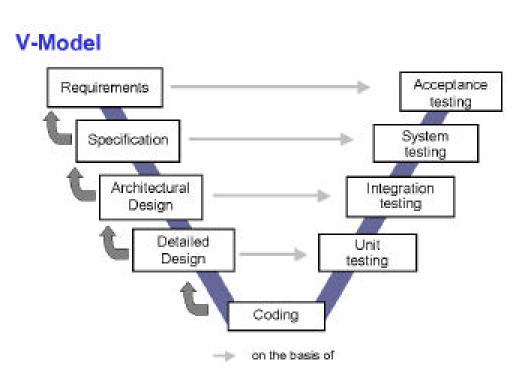
\includegraphics[width=0.5\textwidth]{img/V-model.jpg}
				\caption{Modello a V}
			\end{figure}
	\subsection{Test di validazione}
	\label{test di validazione}
	
		I test di validazione servono per accertarsi che il prodotto realizzato sia conforme alle attese di \PROPONENTE. \\
		Per ognuno vengono indicati i passi necessari all'utente per testare i requisiti associati. Il tracciamento tra i test di validazione e i requisiti correlati viene riportato nel documento \ARdoc.
		\subsubsection{TVF1}
			L'utente verifica di poter creare un account. All'utente è richiesto di:
			\begin{enumerate}
				\item registrare un account;
				\item autenticarsi con i dati del proprio account;
			\end{enumerate}
		\subsubsection{TVF1.1}
			L'utente verifica di potersi autenticare. All'utente è richiesto di:
			\begin{enumerate}
				\item inserire un indirizzo email nel campo apposito;
				\item inserire una password nel campo apposito;
				\item confermare i dati inseriti;
				\item verificare di essere autenticato se i dati inseriti sono corretti;
				\item verificare se viene segnalato ogni eventuale errore durante la procedura di autenticazione. 
			\end{enumerate}
		\subsubsection{TVF1.1.5}
			L'utente verifica che ogni eventuale errore riguardante la procedura di autenticazione interrompa la procedura stessa.
			All'utente è richiesto di:
			\begin{enumerate}
				\item verificare se la procedura viene interrotta quando l'indirizzo email inserito non è già stato registrato;
				\item verificare se la procedura viene interrotta quando la password inserita non coincide con quella associata all'indirizzo email inserito;
				\item verificare che ogni errore nell'inserimento dei dati venga segnalato;
				\item verificare di poter cambiare la password qualora non se la ricordasse. 
			\end{enumerate}
		\subsubsection{TVF1.1.5.4}
			L'utente verifica di poter cambiare la password nel caso non se la ricordasse.
			All'utente è richiesto di:
			\begin{enumerate}
				\item inserire l'indirizzo email con cui si è registrato;
				\item verificare di aver ricevuto un'email all'indirizzo inserito con una nuova password casuale;
				\item verificare che la vecchia password del proprio account venga sostituita con quella nuova inviata per email. 
			\end{enumerate}
		\subsubsection{TVF1.2}
			L'utente verifica di poter registrare un nuovo account.
			All'utente è richiesto di:
			\begin{enumerate}
				\item inserire il proprio indirizzo email nell'apposito campo;
				\item inserire uno username nell'apposito campo;
				\item inserire una password nell'apposito campo;
				\item reinserire la password nell'apposito campo;
				\item confermare i dati inseriti;
				\item verificare che l'account venga registrato con i dati inseriti se non ci sono stati errori, e che l'utente venga autenticato automaticamente;
				\item verificare che vengano segnalati gli errori quando ce ne sono.
			\end{enumerate}
		\subsubsection{TVF1.2.7}
			L'utente verifica che vengano segnalati gli errori quando ce ne sono e, di conseguenza, venga interrotta la procedura di registrazione.
			All'utente è richiesto di:
			\begin{enumerate}
				\item verificare che venga segnalato un errore quando l'indirizzo email inserito non è corretto, in particolare deve contenere una `@', deve finire con un dominio valido e non deve essere già in uso da un altro utente;
				\item verificare che venga segnalato un errore quando lo username inserito non è corretto, in particolare non deve contenere caratteri non alfanumerici e non deve essere già in uso da un altro utente;
				\item verificare che venga segnalato un errore quando la password inserita non è corretta, in particolare deve essere composta da almeno 6 caratteri e da un massimo di 16;
				\item verificare che venga segnalato un errore quando la password reinserita non concide con quella inserita precedentemente.
			\end{enumerate}
		\subsubsection{TVF2}
			L'utente verifica di poter fare il logout.
		\subsubsection{TVF3}
			L'utente verifica di poter fare un percorso quando è disponibile.
			All'utente è richiesto di:
			\begin{enumerate}
				\item giocare il percorso fino a quando non è concluso;
				\item verificare di poter visualizzare i risultati ottenuti durante l'esecuzione del percorso;
				\item verificare di poter salvare i risultati ottenuti.
			\end{enumerate}
		\subsubsection{TVF3.1}
			L'utente verifica di poter giocare il percorso fino alla sua conclusione.
			All'utente è richiesto di:
			\begin{enumerate}
				\item cercare il beacon corrispondente alla prossima stazione;
				\item giocare la prova relativa a quella stazione.
			\end{enumerate}
		\subsubsection{TVF3.1.1}
			L'utente verifica di poter cercare e trovare il beacon della prossima stazione.
			All'utente è richiesto di:
			\begin{enumerate}
				\item verificare se può cominciare a giocare la prova quando trova il beacon;
				\item verificare se i beacon rilevati, ma inutili ai fini della ricerca vengono ignorati dal'app;
				\item verificare di poter chiedere aiuto se non riesce a trovare il beacon o se pensa che ci siano degli errori;
				\item verificare se vengono rilevati dei beacon, esterni al percorso, per segnalare la distanza tra lui e il beacon cercato, e se tale distanza è visualizzata dall'app usando dei valori approssimativi, come delle tacche.
			\end{enumerate}
		\subsubsection{TVF3.1.2}
			L'utente verifica di poter giocare la prova fino alla sua conclusione.
			All'utente è richiesto di:
			\begin{enumerate}
				\item verificare se la prova è una tra quelle previste dall'applicazione;
				\item verificare se vengono visualizzate le istruzioni relative alla prova;
				\item verificare di poter svolgere la prova;
				\item verificare se vengono visualizzati i risultati della prova quando essa viene conclusa;
				\item verificare di poter proseguire il percorso quando la prova giocata non è l'ultima o di poterlo terminare se invece è l'ultima, nel primo caso inoltre l'utente controlla se vengono visualizzate le istruzioni per trovare la stazione successiva.
			\end{enumerate}
		\subsubsection{TVF3.2}
			L'utente verifica di poter visualizzare correttamente i risultati del percorso ottenuti.
			All'utente è richiesto di:
			\begin{enumerate}
				\item verificare se viene visualizzata la durata totale del percorso e se essa viene effettivamente calcolata da quando l'utente accetta di iniziare la prova fino a quando conferma la soluzione dell'ultima prova;
				\item verificare se viene visualizzato il tempo totale impiegato per completare le prove, se esso viene effettivamente calcolato sommando i tempi di ogni prova e se questi ultimi vengono misurati da quando l'utente accetta di iniziare la prova fino alla conferma della sua soluzione;
				\item verificare se viene visualizzato il punteggio totale ottenuto, se esso viene calcolato sommando il punteggio di ogni singola prova, se quest'ultimo viene a sua volta calcolato in base al tipo di prova effettuata e se il risultato ottenuto è il suo nuovo record di quel percorso;
				\item verificare se viene visualizzata la classifica generale relativa a quel percorso e la posizione che l'utente ha raggiunto con quel risultato;
				\item verificare se viene visualizzata la prova con il maggior numero di punti conseguiti;
				\item verificare se viene visualizzata la prova con il minor numero di punti conseguiti.
			\end{enumerate}
		\subsubsection{TVF4}
			L'utente verifica di poter visualizzare le informazioni relative all'app.
			All'utente è richiesto di:
			\begin{enumerate}
				\item verificare di poter visualizzare una schermata con le informazioni generali dell'app;
				\item verificare di poter accedere alla pagina web dell'applicazione tramite un link presente nell'app;
				\item verificare di poter inviare una segnalazione di eventuali errori presenti tramite email.
			\end{enumerate}
		\subsubsection{TVF4.3}
			L'utente verifica di poter giocare la prova fino alla sua conclusione.
			All'utente è richiesto di:
			\begin{enumerate}
				\item verificare se, dopo aver cliccato sul pulsante per le segnalazioni, si apre una nuova email da scrivere tramite il gestore predefinito del dispositivo, dove il destinatario viene impostato automaticamente;
				\item verificare se, dopo aver cliccato il bottone apposito, si apre una schermata dove egli controlla se può selezionare il tipo di errore avuto, verifica se può scegliere la stazione dove pensa si sia presentato l'errore e controlla se, dopo aver confermato i dati, viene inviata un'email all'indirizzo email adibito alle segnalazioni, generata automaticamente in base alle opzioni scelte.
			\end{enumerate}
		\subsubsection{TVF5}
			L'utente verifica di poter visualizzare i risultati dei percorsi effettuati precedentemente.
			All'utente è richiesto di:
			\begin{enumerate}
				\item verificare se, nel caso in cui egli sia autenticato e abbia dei percorsi salvati, viene mostrato l'elenco dei percorsi svolti e se è possibile visualizzare ulteriori informazioni per ognuno di essi;
				\item verificare se, nel caso in cui egli sia autenticato ma non abbia alcun percorso salvato, viene mostrato un invito a svolgere un percorso, oltre ad una spiegazione in cui si informa l'utente che in quella pagina sarà possibile vedere i dati dei percorsi svolti quando verranno salvati;
				\item verificare se, nel caso in cui egli non sia autenticato, viene visualizzato un invito ad autenticarsi, oltre ad una spiegazione dove si informa l'utente che in quella pagina sarà possibile vedere i dati dei percorsi svolti quando verranno salvati.
			\end{enumerate}
		\subsubsection{TVF5.1.1}
			L'utente verifica di poter visualizzare tutte le informazioni relative al percorso salvato scelto.
			All'utente è richiesto di:
			\begin{enumerate}
				\item verificare se viene mostrato il nome del percorso;
				\item verificare se viene visualizzato il nome dell'edificio dove si è svolto il percorso;
				\item verificare se viene mostrata la data in cui si è svolto il percorso;
				\item verificare se viene visualizzato il punteggio totale ottenuto in quel percorso;
				\item verificare se viene mostrato il tempo totale impiegato per poter svolgere il percorso;
				\item verificare se viene visualizzata la posizione attuale nella classifica generale relativa al percorso salvato.
			\end{enumerate}
		\subsubsection{TVF6}
			L'utente verifica di poter visualizzare gli edifici con dei percorsi disponibili più vicini alla sua posizione.
			All'utente è richiesto di:
			\begin{enumerate}
				\item verificare di poter cercare gli edifici inserendo un raggio massimo, oltre a controllare di poter effettivamente visualizzare tutti gli edifici con dei percorsi disponibili nell'area, calcolata in base al valore del raggio immesso, di poter visualizzare informazioni più dettagliate per ognuno di essi e se viene suggerito di aumentare il raggio inserito qualora l'esito della ricerca fosse negativo;
				\item verificare di poter visualizzare tutte le informazioni dell'edificio selezionato.
			\end{enumerate}
		\subsubsection{TVF6.3}
			L'utente verifica di poter visualizzare tutte le informazioni relative all'edificio scelto.
			All'utente è richiesto di:
			\begin{enumerate}
				\item verificare se vengono mostrate le informazioni specifiche dell'edificio;
				\item verificare se viene visualizzato il link alla pagina web dell'edificio;
				\item verificare se vengono mostrati tutti i contatti disponibili per quell'edificio.
			\end{enumerate}
		\subsubsection{TVF6.3.1}
			L'utente verifica di poter visualizzare tutte le informazioni specifiche dell'edificio.
			All'utente è richiesto di:
			\begin{enumerate}
				\item verificare se viene mostrato il nome dell'edificio;
				\item verificare se viene visualizzata la destinazione d'uso della struttura, come ad esempio ``museo di storia egizia'';
				\item verificare se viene mostrato l'indirizzo dell'edificio;
				\item verificare se viene visualizzata una breve descrizione della struttura e del tipo di percorsi presenti.
			\end{enumerate}
		\subsubsection{TVF6.3.3}
			L'utente verifica di poter visualizzare tutti i contatti disponibili dell'edificio.
			All'utente è richiesto di:
			\begin{enumerate}
				\item verificare se viene mostrato il numero di telefono dell'edificio;
				\item verificare se viene visualizzato l'indirizzo email dell'edificio;
				\item verificare se viene mostrato un link alla pagina Facebook dell'edificio nel caso in cui essa esista;
				\item verificare se viene visualizzato un link alla pagina Twitter dell'edificio nel caso in cui essa esista;
				\item verificare se viene mostrato un contatto pubblico di Whatsapp della struttura nel caso in cui esso esista;
				\item verificare se viene visualizzato un contatto pubblico di Telegram della struttura nel caso in cui esso esista.
			\end{enumerate}
		\subsubsection{TVF7}
			L'utente verifica di poter cambiare le proprie credenziali d'accesso.
			All'utente è richiesto di:
			\begin{enumerate}
				\item verificare di poter cambiare la propria password e controllare se essa può effettivamente avere un numero minimo di 6 caratteri e uno massimo di 16;
				\item verificare di poter cambiare il proprio username, di controllare se viene rispettato il vincolo di non poter usare caratteri non alfanumerici per esso e di accertarsi se non è effettivamente possibile utilizzare uno username già in uso da un altro utente;
				\item verificare se l'applicazione informa l'utente quando c'è un errore nei dati inseriti.
			\end{enumerate}
		\subsubsection{TVF8}
			L'utente verifica se viene mostrato un tutorial introduttivo al primo utilizzo dell'app.
		\subsubsection{TVQ1}
			L'utente verifica se viene fornito il manuale per l'utente dell'applicazione.
		\subsubsection{Test di validazione per i requisiti di vincolo} %Se questa sezione viene ritenuta inutile si può pure eliminare
			I requisiti di vincolo rilevati non necessitano di test appositi per motivi diversi:
			\begin{enumerate}
				\item R0V1 è già incluso nella definizione dell'applicazione proposta, inoltre è già verificato nei test dove viene chiesto di controllare se i beacon sono implementati e rilevati correttamente;
				\item R0V2 viene garantito dalla scelta del sistema operativo, visto che Android è specifico per dispositivi mobile.
			\end{enumerate}
		
	\subsection{Test di sistema}
	\label{test di sistema}
		I test di sistema servono per accertarsi che il comportamento dinamico del sistema rispetti i requisiti software individuati e descritti nel documento \ARdoc.
		\subsubsection{Descrizione dei test di sistema}
			% tabella test di sistema esportati da trender
			\begin{tabella}{!{\VRule}l!{\VRule}X[l,b,l]!{\VRule}l!{\VRule}l!{\VRule}}
	\intestazionefourcol{Test}{Descrizione}{Stato}{Requisito}
TS0F1 & Viene verificato che il sistema permetta la creazione e la gestione di un account & N.I & \Req{R0F1} \\ 
TS0F2 & Viene verificato che il sistema permetta la deautenticazione dell'utente & N.I & \Req{R0F2} \\ 
TS0F3 & Viene verificato che il sistema permetta all'utente di giocare un percorso tra quelli disponibili nel luogo in cui si trova & N.I & \Req{R0F3} \\ 
TS0F4 & Viene verificato che il sistema permetta all'utente di visualizzare le informazioni dell'app & N.I & \Req{R0F4} \\ 
TS0F5 & Viene verificato che il sistema permetta all'utente di visualizzare i risultati dei percorsi effettuati precedentemente & N.I & \Req{R0F5} \\ 
TS0F6 & Viene verificato che il sistema permetta all'utente di cercare quali sono gli edifici con percorsi più vicini alla sua posizione & N.I & \Req{R0F6} \\ 
TS0F7 & Viene verificato che il sistema permetta all'utente di modificare le proprie credenziali d'accesso & N.I & \Req{R0F7} \\ 
TS0P1 & Viene verificato che in ogni schermata il tempo di latenza per ottenere una risposta dal server sia minore di 5 secondi, a meno che non vi siano problemi di connessione & N.I & \Req{R0P1} \\ 
TS0P2 & Viene verificato che il tempo di latenza per cambiare la schermata nell'app sia minore di 0.5 secondi, a meno che non sia richiesta l'interazione con il server & N.I & \Req{R0P2} \\ 
TS0Q1 & Viene verificato che il codice rispetti le norme e le metriche delle \NPdoc e della sezione \hyperref[metrichePerIlCodice]{Metriche per il codice} & N.I & \Req{R0Q1} \\ 
TS0Q2 & Viene verificato che i documenti rispettino le norme e le metriche delle \NPdoc e della \hyperref[metrichePerIlCodice]{Metriche per il codice} & N.I & \Req{R0Q2} \\ 
TS0Q3 & Viene verificato che venga fornito il manuale per l'utente & N.I & \Req{R0Q3} \\ 
TS2F8 & Viene verificato che il sistema permetta all'utente di visualizzare un tutorial introduttivo al primo utilizzo dell'app & N.I & \Req{R2F8} \\ 
\rowcolor{white}
\caption{Riepilogo test di sistema}
\end{tabella}
			
			
	\subsection{Test di integrazione}
	\label{test di integrazione}
		I test di integrazione servono per verificare che tutti i diversi componenti del sistema comunichino correttamente tra loro, e che vi sia all'interno del software il flusso di dati atteso. \\
		Verrà utilizzata una strategia di integrazione incrementale per poter sviluppare e verificare più componenti in parallelo. Questo metodo permette di dare priorità ai test relativi alle componenti che vengono ritenute più importanti e quindi sarà possibile partire dalle componenti che soddisfano i requisiti obbligatori fino ad integrarle con quelle che soddisfano i requisiti opzionali. Inoltre permette di restringere la ricerca dell'errore in caso di test fallito, perché molto probabilmente l'errore si trova nel nuovo componente o dalla sua interazione con il sistema corrente. Non si dovrà escludere il caso in cui il test fallisca perché la nuova istanza di test utilizza un campione di input non trattato in precedenza, portando così il sistema a generare l'errore. \\
		L'integrazione delle parti è bottom-up: innanzitutto verranno inserite le componenti con meno dipendenze funzionali e più funzionalità, cioè che corrispondono ai requisiti obbligatori. Di conseguenza queste componenti saranno testate molte volte in modo da ridurre la possibilità che il prodotto finale contenga difetti, e così si otterrà una versione funzionante nel minor tempo possibile. In seguito si risalirà l'albero delle dipendenze fino all'inserimento delle componenti di alto livello. \\
		Questo metodo è più oneroso rispetto ad altri in quanto richiede che venga generato del codice di supporto, sotto forma di driver e stub, che simuli le componenti mancanti, però permette una maggiore copertura perché testa ripetutamente le componenti più importanti.
		
		
	\begin{tabella}{!{\VRule}l!{\VRule}X[l,b,l]!{\VRule}l}
		\intestazionetwocol{Test}{Descrizione}
		TIsavedresults & Verifica che il sistema gestisca correttamente la visualizzazione e il salvataggio dei risultati dei percorsi\\
		 TIdatamanager & Verifica che il sistema gestisca correttamente le richieste dei dati salvati in locale\\
		 TIpathprogress & Verifica che il sistema gestisca correttamente i dati del percorso selezionato e i risultati delle prove giocate\\
		  TIdataserver & Verifica che il sistema gestisca correttamente la modellazione dei dati locali del server \\
		  TIgames & Verifica che il sistema gestisca correttamente il percorso e le prove mentre si sta affrontando un percorso \\
		  TIserver & Verifica che il sistema gestisca correttamente la ricezione, l'elaborazione e la risposta alle richieste del client \\
		   TIlocation & Verifica che il sistema gestisca correttamente l'individuazione e la lettura dei beacon \\
		    TIclient & Verifica che il sistema gestisca ed integri correttamente tutte le parti del client, tra cui l'autenticazione, i percorsi e i servizi vari \\
		     TICLIPS & Verifica che il client e il server comunichino correttamente tra loro \\
		     TIauthentication & Verifica che il sistema gestisca correttamente la registrazione dell'account, il login e la modifica delle proprie credenziali\\ 
		     TIurlrequest & Verifica che il sistema gestisca correttamente le richieste da inviare la server\\
		     TIviewcontroller & Verifica che il sistema gestisca correttamente le pagine dell'applicazione e le risposte agli input dell'utente\\
		      TIutility & Verifica che il sistema gestisca correttamente le view generali dell'app\\
		       TIbuilding & Verifica che il sistema gestisca correttamente le view e le interazioni dell'utente riguardanti gli edifici abilitati e i relativi percorsi\\
		       TIurlrequesthandler & Verifica che il sistema gestisca correttamente le richieste del client e le risposte da inviare\\
		       TIdata & Verifica che il sistema gestisca correttamente la modellazione dei dati in locale\\
		       \end{tabella}


		
		
\appendix


\section{Resoconto dell’attività di verifica}
\label{resocontoDellAttivitaDiVerifica}
	\subsection{Periodo di Analisi e Management}
	\label{periodoDiAnalisiEManagement}
		\subsubsection{Processi}
		\label{processiAM}
			Sono riportati ora i valori di Schedule Variance e Budget Variance per le attività del Periodo di Analisi e Management.
			\begin{tabella}{!{\VRule}l!{\VRule}l!{\VRule}l!{\VRule}}
				\intestazionethreecol{Attività}{Schedule Variance}{Budget Variance}
				\ARdoc & \euro\ -10 & \euro\ +15 \\
				\Gldoc & \euro\ 0 & \euro\ 0 \\
				\NPdoc & \euro\ -5 & \euro\ +10 \\
				\PPdoc & \euro\ 0 & \euro\ +20 \\
				\PQdoc & \euro\ +5 & \euro\ -10 \\
				\SFdoc & \euro\ -10 & \euro\ 0 \\
				
				\hiderowcolors
				\caption{Esiti verifica sui processi - Periodo di Analisi e Management}
			\end{tabella}
			In totale sono stati registrati:
			\begin{itemize}
				\item \textbf{Schedule Variance:}\ \euro\ -20;
				\item \textbf{Budget Variance:}\ \euro\ +35.
			\end{itemize}
			Dai valori ottenuti si nota subito che in alcuni casi è stata prevista qualche ora di attività in più rispetto al necessario. Questo ha portato ad avere una Budget Variance positiva, mentre la causa di questo fatto è da ricercare nell'inesperienza del gruppo, che ha portato ad una valutazione leggermente errata del carico di lavoro necessario. Sempre a causa della poca esperienza del gruppo la Schedule Variance è risultata negativa, perché alcune attività si sono concluse leggermente in ritardo rispetto alle aspettative. La causa di questo fatto è da ricercare nell'organizzazione da parte dei membri del gruppo dei propri impegni, da cui sono derivati leggeri ritardi che si sono sommati. Il risultato comunque rientra nel limite ottimale, che sarebbe di \euro\ -144.
			%Nota sull'interpretazione della giustificazione sopra: quello che volevo indicare sopra per la Budget Variance è che inizialmente ci sono stati leggeri ritardi, che comunque poi sono stati compensati alla fine (vista anche la consegna anticipata rispetto al previsto)
		\subsubsection{Documenti}
		\label{documentiAM}
			Sono riportati qui i valori dell'indice Gulpease per ogni documento presente durante l'attività di analisi nel Periodo di Analisi e Management. Un documento è considerato valido soltanto se rispetta le metriche descritte secondo la sezione \hyperref[indiceGulpease]{Indice Gulpease}.
			\begin{tabella}{!{\VRule}l!{\VRule}c!{\VRule}c!{\VRule}}
				\intestazionethreecol{Documento}{Valore}{Esito}
				\ARdoc & 66 & Superato\\
				\Gldoc & 53 & Superato\\
				\NPdoc & 56 & Superato\\
				\PPdoc & 53 & Superato\\
				\PQdoc & 60 & Superato\\
				\SFdoc & 61 & Superato\\
				
				\hiderowcolors
				\caption{Esiti verifica documenti - Periodo di Analisi e Management}
			\end{tabella}
	\subsection{Periodo di Analisi di Dettaglio}
	\label{periodoDiAnalisiDiDettaglio}
		\subsubsection{Processi}
		\label{processiAD}
			Sono riportati ora i valori di Schedule Variance e Budget Variance per le attività del Periodo di Analisi di Dettaglio.
				\begin{tabella}{!{\VRule}l!{\VRule}c!{\VRule}c!{\VRule}}
				\intestazionethreecol{Attività}{Schedule Variance}{Budget Variance}
				\ARdoc & \euro\ -20 & \euro\ -25 \\
				\Gldoc & \euro\ 0 & \euro\ 0 \\
				\NPdoc & \euro\ +5 & \euro\ +5 \\
				\PPdoc & \euro\ -10 & \euro\ -10 \\
				\PQdoc & \euro\ 0 & \euro\ -5 \\
				\SFdoc & \euro\ 0 & \euro\ 0 \\
				
				\hiderowcolors
				\caption{Esiti verifica sui processi - Periodo di Analisi di Dettaglio}
			\end{tabella}
			In totale sono stati registrati:
			\begin{itemize}
				\item \textbf{Schedule Variance:}\ \euro\ -25;
				\item \textbf{Budget Variance:}\ \euro\ -35.
			\end{itemize}
			Dai valori ottenuti si nota subito che il lavoro richiesto per eseguire le attività è stato maggiore di quello pianificato. Questo perché le modifiche necessarie si sono rivelate essere più del previsto, soprattutto per quanto riguarda l'Analisi dei Requisiti. Di conseguenza la Budget Variance e la Schedule Variance sono risultate negative, ma comunque al di sotto del limite ottimale di \euro\ -65.
		\subsubsection{Documenti}
		\label{documentiAD}
			Sono riportati qui i valori dell'indice Gulpease per ogni documento presente durante l'attività di analisi nel Periodo di Analisi di Dettaglio. Un documento è considerato valido soltanto se rispetta le metriche descritte secondo la sezione \hyperref[indiceGulpease]{Indice Gulpease}.
			\begin{tabella}{!{\VRule}l!{\VRule}c!{\VRule}c!{\VRule}}
				\intestazionethreecol{Documento}{Valore}{Esito}
				\ARdoc & 85 & Superato\\
				\Gldoc & 54 & Superato\\
				\NPdoc & 51 & Superato\\
				\PPdoc & 62 & Superato\\
				\PQdoc & 61 & Superato\\
				\SFdoc & 61 & Superato\\
				
				\hiderowcolors
				\caption{Esiti verifica documenti - Periodo di Analisi di Dettaglio}
			\end{tabella}
	\subsection{Periodo di Progettazione Architetturale}
	\label{periodoDiProgettazioneArchitetturale}
		\subsubsection{Processi}
		\label{processiPA}
			Sono riportati ora i valori di Schedule Variance e Budget Variance per le attività del Periodo di Progettazione Architetturale.
				\begin{tabella}{!{\VRule}l!{\VRule}c!{\VRule}c!{\VRule}}
				\intestazionethreecol{Attività}{Schedule Variance}{Budget Variance}
				\ARdoc & \euro\ +20 & \euro\ +20 \\
				\Gldoc & \euro\ +5 & \euro\ 0 \\
				\NPdoc & \euro\ +10 & \euro\ +15 \\
				\PPdoc & \euro\ -5 & \euro\ 0 \\
				\PQdoc & \euro\ -5 & \euro\ 0 \\
				\STdoc & \euro\ -20 & \euro\ -50 \\
				
				\hiderowcolors
				\caption{Esiti verifica sui processi - Periodo di Progettazione Architetturale}
			\end{tabella}
			In totale sono stati registrati:
			\begin{itemize}
				\item \textbf{Schedule Variance:}\ \euro\ +5;
				\item \textbf{Budget Variance:}\ \euro\ -15.
			\end{itemize}
			Dai valori ottenuti si nota subito che le attività si sono concluse al massimo leggermente dopo i tempi previsti, ad eccezione della Specifica Tecnica che ha subito notevoli ritardi.\\
			Questo ha portato ad avere una Schedule Variance leggermente positiva perché il tempo risparmiato ha compensato quello perso per la Specifica Tecnica, in particolare sono risultate importanti le ore dedicate nella fase precedente perchè ha permesso di avere dei documenti praticamente già terminati.\\
			Al contrario la budget Variance è risultata negativa ma comunque al di sotto del limite ottimale di \euro\ -204. Questo perché le ore di lavoro previste per tutti i documenti sono risultate sufficienti o addirittura eccessive, ma la Specifica Tecnica ha richiesto molte più ore del previsto.\\
			I dati negativi relativi a questo documento sono da ricercare sempre nell'inesperienza del gruppo, che ha portato a sopravvalutare non di poco i tempi e le ore richiesti per portarlo a termine, in particolare per quanto riguarda la progettazione delle classi.
		\subsubsection{Documenti}
		\label{documentiPA}
			Sono riportati qui i valori dell'indice Gulpease per ogni documento presente durante l'attività di analisi nel Periodo di Progettazione Architetturale. Un documento è considerato valido soltanto se rispetta le metriche descritte secondo la sezione \hyperref[indiceGulpease]{Indice Gulpease}.
			\begin{tabella}{!{\VRule}l!{\VRule}c!{\VRule}c!{\VRule}}
				\intestazionethreecol{Documento}{Valore}{Esito}
				\ARdoc & 84  & Superato\\
				\Gldoc & 54 & Superato\\
				\NPdoc & 71 & Superato\\
				\PPdoc & 51 & Superato\\
				\PQdoc & 61 & Superato\\
				\STdoc & 86 & Superato\\
				
				\hiderowcolors
				\caption{Esiti verifica documenti - Periodo di Progettazione Architetturale}
			\end{tabella}
		\subsection{Periodo di Progettazione di Dettaglio e Codifica}
			\label{periodoDiProgettazioneDiDettaglioECodifica}
				\subsubsection{Processi}
				\label{processiPDC}
					Sono riportati ora i valori di Schedule Variance e Budget Variance per le attività del Periodo di Progettazione di Dettaglio e Codifica.
						\begin{tabella}{!{\VRule}l!{\VRule}c!{\VRule}c!{\VRule}}
						\intestazionethreecol{Attività}{Schedule Variance}{Budget Variance}
						\ARdoc & \euro\ +10 & \euro\ +10 \\
						\DPdoc & \euro\ -20 & \euro\ -25 \\
						\Gldoc & \euro\ +5 & \euro\ +10 \\
						\MUdoc & \euro\ +20 & \euro\ +15 \\
						\NPdoc & \euro\ -5 & \euro\ 0 \\
						\PPdoc & \euro\ +10 & \euro\ +20 \\
						\PQdoc & \euro\ +5 & \euro\ 0 \\
						\STdoc & \euro\ -10 & \euro\ -15 \\
						
						\hiderowcolors
						\caption{Esiti verifica sui processi - Periodo di Progettazione di Dettaglio e Codifica}
					\end{tabella}
					In totale sono stati registrati:
					\begin{itemize}
						\item \textbf{Schedule Variance:}\ \euro\ +15;
						\item \textbf{Budget Variance:}\ \euro\ +10.
					\end{itemize}
					Dai valori ottenuti si nota subito che le attività sono state concluse in anticipo rispetto alle previsioni, e con una quantità di lavoro minore di quella prevista. I valori di Schedule Variance e di Budget Variance sono risultati quindi positivi, perché la correzione di alcuni documenti ha richiesto meno tempo del previsto. Questo risultato è da cercarsi anche nel maggior carico di lavoro richiesto dalla parte di codifica, che quindi ha portato il gruppo a sistemare presto i documenti. 
				\subsubsection{Documenti}
				\label{documentiPDC}
					Sono riportati qui i valori dell'indice Gulpease per ogni documento presente durante l'attività di analisi nel Periodo di Progettazione di Dettaglio e Codifica. Un documento è considerato valido soltanto se rispetta le metriche descritte secondo la sezione \hyperref[indiceGulpease]{Indice Gulpease}.
					\begin{tabella}{!{\VRule}l!{\VRule}c!{\VRule}c!{\VRule}}
						\intestazionethreecol{Documento}{Valore}{Esito}
						\ARdoc & 84  & Superato\\
						\DPdoc & & Superato\\
						\Gldoc & 54 & Superato\\
						\MUdoc & & Superato\\
						\NPdoc & 71 & Superato\\
						\PPdoc & 51 & Superato\\
						\PQdoc & 61 & Superato\\
						\STdoc & 86 & Superato\\
						
						\hiderowcolors
						\caption{Esiti verifica documenti - Periodo di Progettazione di Dettaglio e Codifica}
					\end{tabella}

\section{Esito delle revisioni}
\label{sec:B}
	Durante lo sviluppo del progetto ci saranno quattro revisioni a cui sottoporsi. Il \gl{committente} segnalerà gli errori riscontrati fornendo una valutazione generica dell'andamento del progetto ed una dettagliata per ogni documento. Si elencano di seguito le modifiche apportate in seguito alle revisioni.
	\subsection{Revisione dei Requisiti}
	\label{sec:B.1}
		\begin{itemize}
			\item \textbf{Studio di fattibilità:}\ sono stati corretti gli acronimi scritti in maniera errata.
			\item \textbf{Norme di progetto:}\ nel documento sono state aggiunte le sezioni che erano state impropriamente inserite nel documento \PQdocRR.
			\item \textbf{Analisi dei Requisiti:}\ sono stati modificati numerosi casi d'uso, cambiando ad esempio la descrizione, lo scenario principale e il padre. Inoltre sono stati aggiunti parecchi casi d'uso, mentre altri sono stati eliminati. Sono stati modificati anche numerosi requisiti sia come conseguenza delle modifiche dei casi d'uso sia per le segnalazioni ricevute. Sono stati aggiunti tanti requisiti e ne sono stati eliminati alcuni.
			\item \textbf{Piano di Progetto:}\ sono state aggiunte le sezioni sul'Analisi dinamica dei rischi e sono stati cambiati i nomi dei periodi.
			\item \textbf{Piano di Qualifica:}\ il documento è stato completamente rivisto a seguito delle segnalazioni. Sono state aggiunte altre metriche, soprattutto per la verifica dei processi, ed è stata ampliata l'appendice con i risultati della verifica.
			%se anche altri documenti vengono modificati, tipo il Glossario, bisogna aggiungere qua cosa è stato modificato
		\end{itemize}

\end{document}
